% !TeX program = xelatex
\documentclass[12pt]{article}
\usepackage[left=3cm,top=3cm,right=2cm,bottom=2cm]{geometry}% //margens conforme a abnt se precisar
\usepackage{graphicx} % Required for inserting images
\usepackage{nameref} % Must come after hyperref
\usepackage{fontspec}
\usepackage{makecell} % Add this in the preamble
\usepackage{hyperref}
\usepackage{titlecaps}
\usepackage{titlesec}
\usepackage{tocloft}  % For customizing ToC
\usepackage{textcomp}
 \usepackage{gensymb}
\usepackage{tabularx}
\usepackage{mathtools}
\DeclarePairedDelimiter\abs{\lvert}{\rvert}
\usepackage{indentfirst}
\usepackage{url}          % For handling URLs

\usepackage{enumitem}
\usepackage{fancyhdr}

\usepackage{floatrow}
\floatsetup[table]{capposition=top}
\floatsetup[figure]{capposition=top}

\usepackage{caption}    % For modifying caption styles
%\DeclareCaptionFont{custom}{\fontsize{12pt}{14pt}\selectfont}
%\captionsetup{font=custom} 

% If you want a dash instead of a space, use:
\captionsetup[figure]{labelsep=endash} % Makes it "Figure X –"

\captionsetup[table]{labelsep=endash} % Removes ":" after "Table X"


% Fix section number to be just arabic (1, 2, ...)
\renewcommand{\thesection}{\arabic{section}}

% Add dot after section number in heading
%\titlelabel{\thetitle.\quad}

\renewcommand{\numberline}[1]{#1\hspace{0.8em}}  % controla espaçamento depois do número

\usepackage{setspace}  % Import setspace package
\onehalfspacing  % Sets line spacing to 1.5

% Load biblatex with abnt style and biber backend

\usepackage[
backend=biber,
style=abnt,
maxcitenames=3,
sorting=nyt,
language=brazilian,
repeatfields=true
]{biblatex}

%\renewcommand{\abntetalchar}{\textit{et al.}}

% Custom macro to show "Disponível em:" and "Acesso em:"
\renewbibmacro*{url} {
  \iffieldundef{url}{}{
    \printtext{Disponível em:} \space \printfield{url}
  }
}

\addbibresource{referencias.bib}

\DeclareFieldFormat[inproceedings]{title}{\textbf{#1}}

\renewbibmacro*{name:andothers}{% Based on name:andothers from biblatex.def
  \ifboolexpr{
    test {\ifnumequal{\value{listcount}}{\value{liststop}}}
    and
    test \ifmorenames
  }
    {\ifnumgreater{\value{liststop}}{1}
       {\finalandcomma}
       {}%
     \andothersdelim\bibstring[\emph]{andothers}}
    {}}


% Redefining maketitle to swap order
\makeatletter
\renewcommand{\maketitle}{
  \begin{center}
    {\@author}  % Author first

    \vspace{6\baselineskip}
    
    {\@title} % Title second
    
    \vspace{2\baselineskip}

  \end{center}
}
\makeatother

% Redefine the URL command to remove angle brackets
%\renewcommand{\UrlLeft}{}
%\renewcommand{\UrlRight}{}

\hypersetup{
    colorlinks=true,        % Enable colored links
    linkcolor=black,        % No color for internal links like references
    citecolor=black,        % No color for citation links
    urlcolor=blue           % Keep color for external URLs
}

% Remove inverted symbols around URL
\DeclareFieldFormat{url}{\url{#1}}

%\pagestyle{fancy}
%\fancyhf{} % Clear header and footer
%\fancyhead[R]{\thepage} % Place page number in the top right
%\renewcommand{\headrulewidth}{0pt} % Remove the line at the top

% Add dots (leaders) between the title and page number in the ToC
%\renewcommand{\cftsecleader}{\cftdotfill{\cftdotsep}}
% Customize the online entry type to reorder "Disponível em" and "Acesso em"
% Rename "Contents" to "Súmario"
\renewcommand{\contentsname}{\MakeUppercase{Sumário}}
\renewcommand{\abstractname}{Resumo}
\renewcommand{\figurename}{Figura} %Troca "Figure" por "Figura" 
\renewcommand{\listfigurename}{\MakeUppercase{Lista de Figuras}}
\renewcommand{\listtablename}{\MakeUppercase{Lista de Tabelas}}
\renewcommand{\tablename}{Tabela}


\title{AVALIAÇÃO DO DESEMPENHO ENERGÉTICO DE SISTEMAS AUTOMOTIVOS DE CONDICIONAMENTO DE AR}
\author{GUSTAVO ROHRICHT MACHADO}
\date{April 2025}

%hyphenations
\hyphenation{con-di-ções}  % Allows LaTeX to break "condições" properly
\hyphenation{vo-lu-mé-tri-ca}  
\hyphenation{gran-de-zas}
\hyphenation{ins-tru-men-ta-da}
\hyphenation{pa-râ-me-tros}
\hyphenation{des-car-ga}
\hyphenation{tem-pe-ra-tu-ras}
\hyphenation{is-to}
\hyphenation{cons-tan-te}
\begin{document}

%--------------------------------------------------

\singlespacing  % Disable 1.5 spacing for this page
\pagestyle{empty}  % Hide page numbers for multiple pages

\setmainfont{Arial}
\begin{figure}
    \centering
    
\includegraphics[width=2.39cm,height=3.3cm]{Logo UFSC/logoUFSC.png}
    \label{fig:elogoUFSC}    
\end{figure}

\begin{center}
    UNIVERSIDADE FEDERAL DE SANTA CATARINA

    CENTRO TECNOLÓGICO DE JOINVILLE  
\end{center}
    \vspace{2\baselineskip}
    
\maketitle

\begin{center}
    Orientador: Prof. Diogo Lôndero da Silva, Dr.Eng.

    \vspace{12\baselineskip}

    Joinville

    2025
    
\end{center}


%--------------------------------------------------

\onehalfspacing  % Sets line spacing to 1.5
\begin{center}
    \textbf{RESUMO}
\end{center}

{\noindent Este relatório apresenta uma análise experimental do comportamento transiente de um sistema de condicionamento de ar automotivo sob diferentes condições de operação. Foram medidos temperatura, pressão, umidade relativa e vazão mássica em pontos estratégicos do sistema durante cinco ensaios com perturbações provocadas pela variação da rotação do compressor e da vazão de ar do ventilador do evaporador. Observou-se que o aumento da vazão de ar gera resposta oscilatória, com sobressinal de aproximadamente 6\%, enquanto alterações na rotação do compressor resultam em resposta suave, sem sobressinal. As maiores histereses ocorreram na descarga do compressor, atingindo 16\% na forma normalizada. Quanto ao desempenho, o COP reduziu 43\% com aumento da vazão de ar e aumentou 22\% com sua redução. Foi identificada histerese no COP, com diminuição de cerca de 11\% durante a elevação da rotação do compressor e aumento de aproximadamente 12\% na redução desta.
\\\\
\noindent \textbf{Palavras-chave}: Coeficiente de desempenho (COP); Comportamento transiente; Condicionamento de ar automotivo; Histerese. 
}
\newpage

\begin{center}
    \textbf{ABSTRACT}
\end{center}

{\noindent This report presents an experimental analysis of the transient behavior of an automotive air conditioning system under different operating conditions. Temperature, pressure, relative humidity, and mass flow rate were measured at strategic points of the system during five tests with disturbances caused by variations in the compressor rotational speed and in the evaporator fan airflow rate. It was observed that increasing the airflow rate produces an oscillatory response, with an overshoot of approximately 6\%, while changes in the compressor speed result in a smooth response without overshoot. The largest hysteresis occurred at the compressor discharge, reaching 16\% in normalized form. Regarding performance, the COP decreased by 43\% with increased airflow rate and increased by 22\% with its reduction. Hysteresis in COP was also identified, with a decrease of about 11\% during the increase in compressor speed and an increase of approximately 12\% during its reduction.
\\\\
\noindent \textbf{Keywords}: Automotive air conditioning; Coefficient of performance (COP); Hysteresis; Transient behavior.
}

\onehalfspacing

%--------------------------------------------------

\onehalfspacing
\newpage
\begin{center}
    \textbf{Agradecimentos}
\end{center}

{

Ao Laboratório de Refrigeração Veicular (REVE) da Universidade Federal de Santa Catarina (UFSC) pelo suporte na realização deste projeto, ao Conselho Nacional de Desenvolvimento Científico e Tecnológico (CNPQ) e a Fundação de Amparo à Pesquisa e Inovação do Estado de Santa Catarina (Fapesc) pelo apoio na financeiro para aquisição dos equipamentos necessário para a construção do aparato.
O presente trabalho foi realizado com apoio do CNPq, Conselho Nacional de Desenvolvimento Científico e Tecnológico - Brasil.
}

%--------------------------------------------------

\include{AntesdoTexto/4-Listas e Sumário}

%--------------------------------------------------

\newpage
\pagenumbering{arabic}  % Resume numbering
\setcounter{page}{8}  %
\pagestyle{plain}  % Force page number to appear again

\pagestyle{fancy}
\fancyhf{}  % Clear header and footer
\fancyfoot[R]{\thepage}  % Move page number to lower right
\renewcommand{\headrulewidth}{0pt}  % Remove header line
\renewcommand{\footrulewidth}{0pt}  % Remove footer line

%--------------------------------------------------

\section{INTRODUÇÃO}

Em decorrência da popularização dos veículos de carroceria fechada, constatou-se a necessidade do desenvolvimento de sistemas voltados à garantia do conforto térmico de seus ocupantes. 
Assim, na década de 1930, iniciou-se nos Estados Unidos o desenvolvimento do sistema de condicionamento de ar em veículos, com o primeiro registro de comercialização do primeiro veículo com sistema de condicionamento de ar nativo de fábrica, o Packard 180 (One-Eighty) produzido pela fabricante Packard Motor Car \cite{bhatti1999}, o qual é apresentado na Figura \ref{fig:sistemaMAC}, assim como a disposição dos principais componentes necessários para o funcionamento do sistema de condicionamento de ar no veículo.
\\

\begin{figure}[h]
    \centering
    
    \caption{ Representação do Sistema MAC (Mobile Air Conditioning) no Veículo Packard 180}
    
    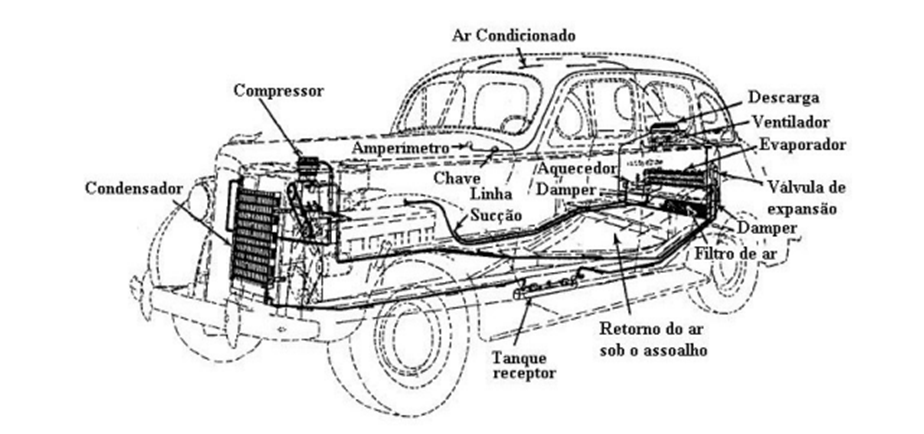
\includegraphics[width=15.65cm, height=7.35cm]{FigurasdoTexto/sistemaMAC.png}
    
     \vspace{5pt}  % Add space before source
    {\footnotesize Fonte: Bhatti adaptado por Santos (2005).}  % Source text in smaller font
    \label{fig:sistemaMAC}
\end{figure}

Atualmente, o Brasil está bem ranqueado na produção de veículos com sistema de condicionamento de ar nativo de fábrica, sendo o maior montador de veículos com ar condicionado da América do Sul e o 10º maior da América Latina com cerca de dois milhões de unidades de passeio \cite{dasilva2024}. Analisando o ano de novembro de 2024, a frota de veículos somente no Brasil era de 123,5 milhões, aproximadamente 63 milhões são automóveis, o que equivale a cerca de 51,2\%  \cite{ministerio2024}.
\newpage
Esse sistema de condicionamento de ar automotivo consome uma parte significativa da potência do motor durante a operação do veículo, com sua eficiência de refrigeração diretamente relacionada à capacidade de carga térmica. Em média, o ar-condicionado é utilizado entre 43\% e 49\% do tempo total de uso do veículo \cite{farrington2000}.

O sistema por compressão mecânica de vapor utilizado em sistemas veiculares, segundo  \textcite{dasilva2016}, possui uma estrutura semelhante à dos sistemas de condicionamento de ar mecânico convencionais. Os principais componentes desses sistemas incluem trocadores de calor, um compressor e uma válvula ou dispositivo de expansão.

O princípio de funcionamento dos sistemas de condicionamento de ar e de refrigeração por compressão mecânica de vapor é compreendido pela operação dos quatro principais componentes: o compressor promove o escoamento do refrigerante ao longo do sistema, elevando a pressão e temperatura do fluido refrigerante, enquanto isso, o evaporador e condensador atuam como trocadores de calor, absorvendo e rejeitando o calor do ambiente a ser resfriado, e o dispositivo de expansão realiza a expansão isentrópica do fluido refrigerante, causando a redução da temperatura do mesmo \cite{junior2023}.

Em geral, as propriedades dos sistemas veiculares não permanecem constantes durante toda a operação de um veículo, sendo precedidas por um regime transitório em que as propriedades do sistema variam devido a fatores externos. Em veículos com motores a combustão interna o compressor é acionado pelo próprio motor do veículo, de forma que a sua rotação depende da rotação do motor e normalmente não está correlacionada com a carga térmica do sistema de condicionamento de ar. Tal condição, devido aos sucessivos transientes na operação do compressor, resulta em desafios para o dimensionamento dos componentes e implementação de uma lógica de controle. Além disso, deve-se levar em conta o ciclo tradicional de controle da temperatura do veículo, no qual o sistema é acionado e desligado continuamente com o objetivo de atingir uma temperatura determinada \cite{juliani2017}.

Durante a operação nesse tipo de regime, os componentes podem apresentar não uniformidade das condições internas, a vazão mássica do refrigerante varia continuamente, resultando em mudanças na distribuição do refrigerante entre os componentes do sistema assim como a variação do superaquecimento e o ponto de operação do dispositivo de expansão, que se ajusta e regula continuamente para a operação \cite{rangel2007}. Devido a esse motivo, faz-se necessária a realização de mais estudos sobre o comportamento do sistema durante o regime transiente com o intuito de aumentar a eficiência do sistema de condicionamento de ar.

\subsection{OBJETIVOS}

\subsubsection{Objetivo Geral}

Análise experimental do comportamento transiente de um sistema de condicionamento de ar automotivo e de seu ciclo de histerese para avaliar o seu efeito sobre o coeficiente de performance (COP), considerando diferentes condições de operação.

\subsubsection{Objetivos Específicos}

Para alcançar o objetivo geral, os objetivos específicos propostos são:

\begin{enumerate}[label=\arabic*]
    \item Revisão bibliográfica e obtenção de dados do sistema de referência;
    
    \item Identificar modos para controle da rotação do compressor;
    
    \item Adaptação do aparato experimental;
    
    \item Estimativa das incertezas experimentais;

    \item Elaboração do plano experimental;
    
    \item Realização dos experimentos e obtenção da base de dados experimental;
    
    \item Quantificar as histereses associadas às diferentes perturbações.

\end{enumerate}


%--------------------------------------------------

\include{Sections/2-MateriaisMétodos}

%--------------------------------------------------

\include{Sections/3-ResultadosDiscussão}

%--------------------------------------------------

\include{Sections/4-Conclusão}

%--------------------------------------------------

\addcontentsline{toc}{section}{REFERÊNCIAS}
\renewcommand{\refname}{\MakeUppercase{Referências}}
\printbibliography

\end{document}